\begin{frame}
\hypertarget{Share}{}
\hyperlink{Count}{\beamergotobutton{Count}}
\begin{figure}
    \centering
    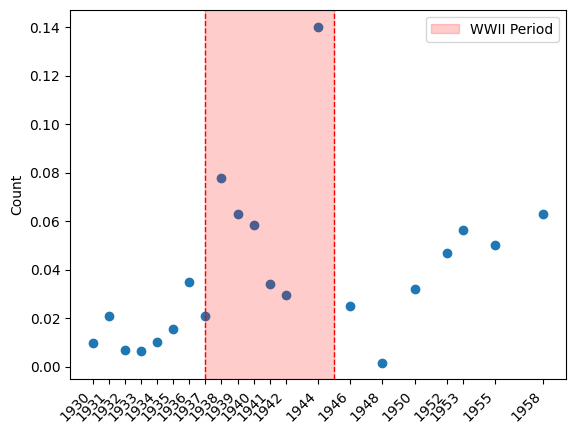
\includegraphics[width=\linewidth]{Background/FemaleEntryShare.png}
    \label{fig:department-figure}
\end{figure}
\end{frame}

\begin{frame}
\hypertarget{Department}{}
\hyperlink{Descriptive}{\beamergotobutton{Descriptive}}
\begin{figure}
    \centering
    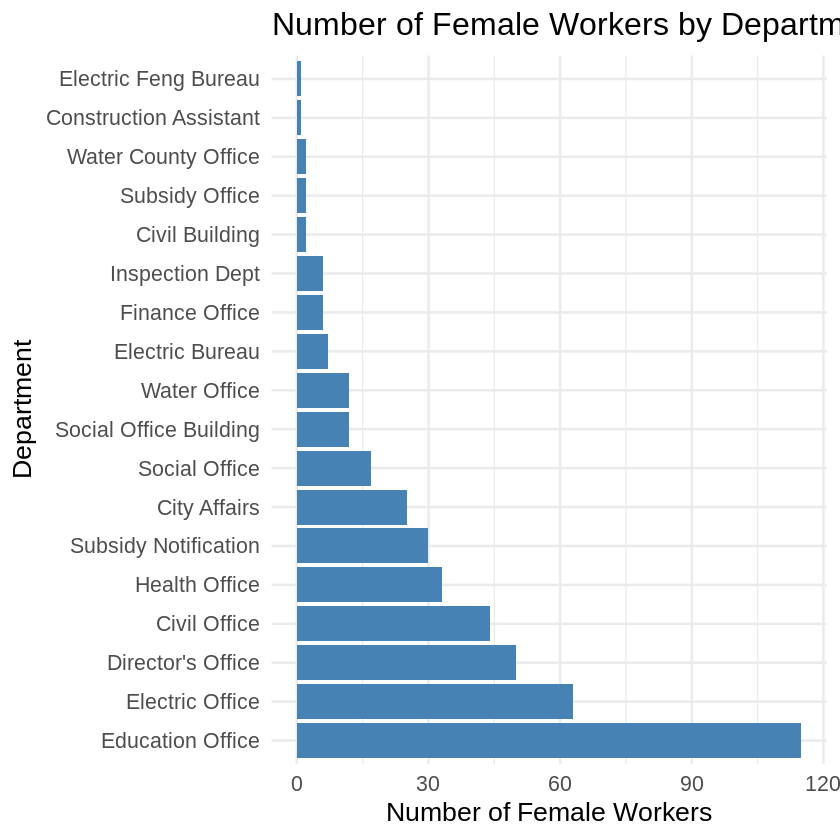
\includegraphics[width=0.8\linewidth]{Background/FemaleCountBar.png}
    \caption{Number of Female Workers by Department}
    \label{fig:department-figure}
\end{figure}
\end{frame}

\begin{frame}
\hypertarget{Occupation}{}
\hyperlink{Descriptive}{\beamergotobutton{Descriptive}}
\begin{figure}
    \centering
    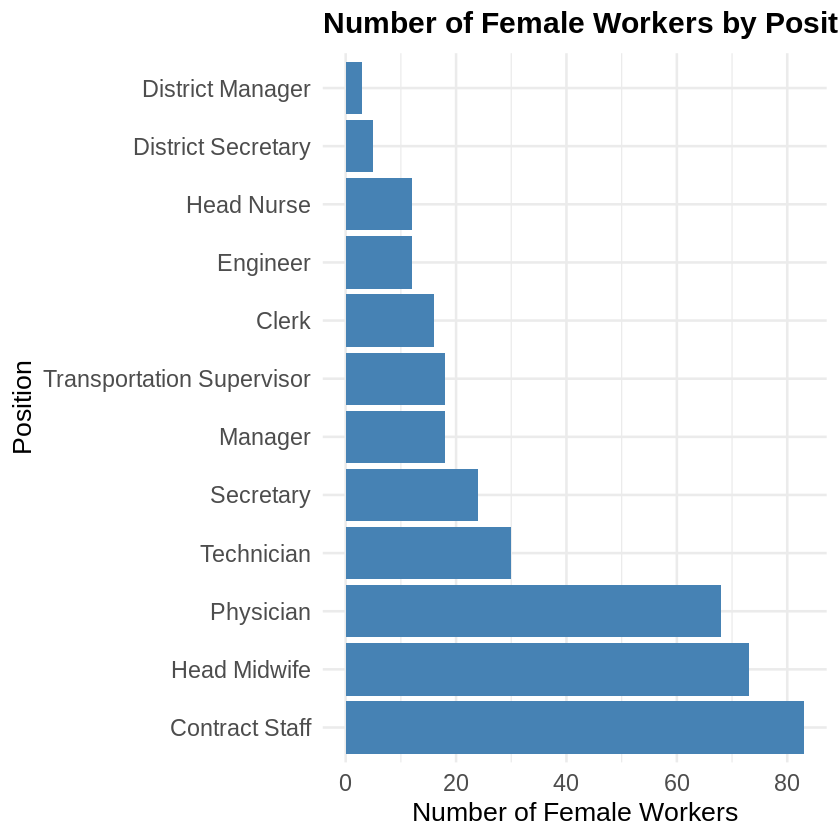
\includegraphics[width=0.8\linewidth]{Background/FemaleCountPosition.png}
    \caption{Number of Female Workers by Occupation}
    \label{fig:occupation-figure}
\end{figure}
\end{frame}

\begin{frame}
\hypertarget{TimeSeries}{}
\begin{figure}
    \centering
    \caption{Number of Female workers in the Tokyo Civil Service}
    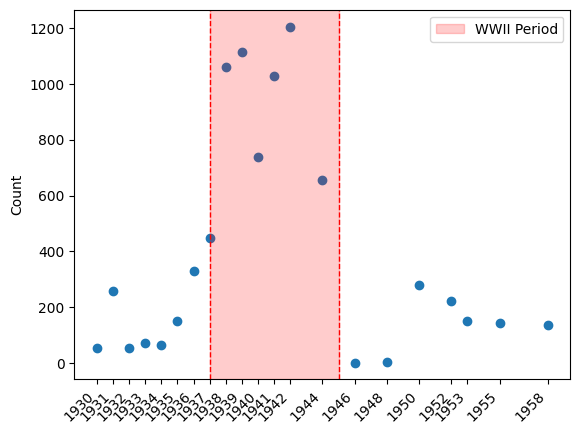
\includegraphics[width=\linewidth]{Background/FemaleEntry.png}
    \label{fig:time-series-figure}
\end{figure}
\hyperlink{Descriptive}{\beamergotobutton{Descriptive}}
\end{frame}
